%%%%%%%%%%%%%%%%%%%%%%%%
%
% $Autor: Wings $
% $Datum: 2020-07-24 09:05:07Z $
% $Pfad: GDV/Vortraege/latex - Ausarbeitung/Kapitel/Einleitung.tex $
% $Version: 4732 $
%
%%%%%%%%%%%%%%%%%%%%%%%%

\chapter{Positioning Within Standard Reference Architectures}

This solution aligns with several modern frameworks and architectures:

\begin{itemize}
	\item \textbf{Smart-City:} The analytics align with secure data handling standards in urban development contexts, ensuring efficient and secure information exchange in large-scale urban projects..
	\item \textbf{IIoT/IIRA:} The approach supports reliability and security within industrial systems, adhering to frameworks like the Industrial Internet Reference Architecture (IIRA) for seamless integration and operational consistency, refer figure ~\ref{RAMI_IIRA}.
	\item \textbf{RAMI 4.0:} Within the Reference Architecture Model for Industry 4.0 (RAMI 4.0), the analytics are positioned in the \SHELL{"Information Layer"}, where data processing, analysis, and anomaly detection occur. It also contributes to the "Functional Layer" by enabling actionable insights and decision-making based on real-time monitoring, refer figure ~\ref{RAMI_IIRA}.
	\item \textbf{ISO Standards Compliance:} The analytics are developed in alignment with international standards such as ISO 27001, ensuring robust security practices and data protection.
	\item \textbf{Cybersecurity Frameworks:} Incorporating principles from the NIST Cybersecurity Framework, the analytics bolster detection, prevention, and response mechanisms for threats.
\end{itemize}

\begin{figure}
	\begin{center}
		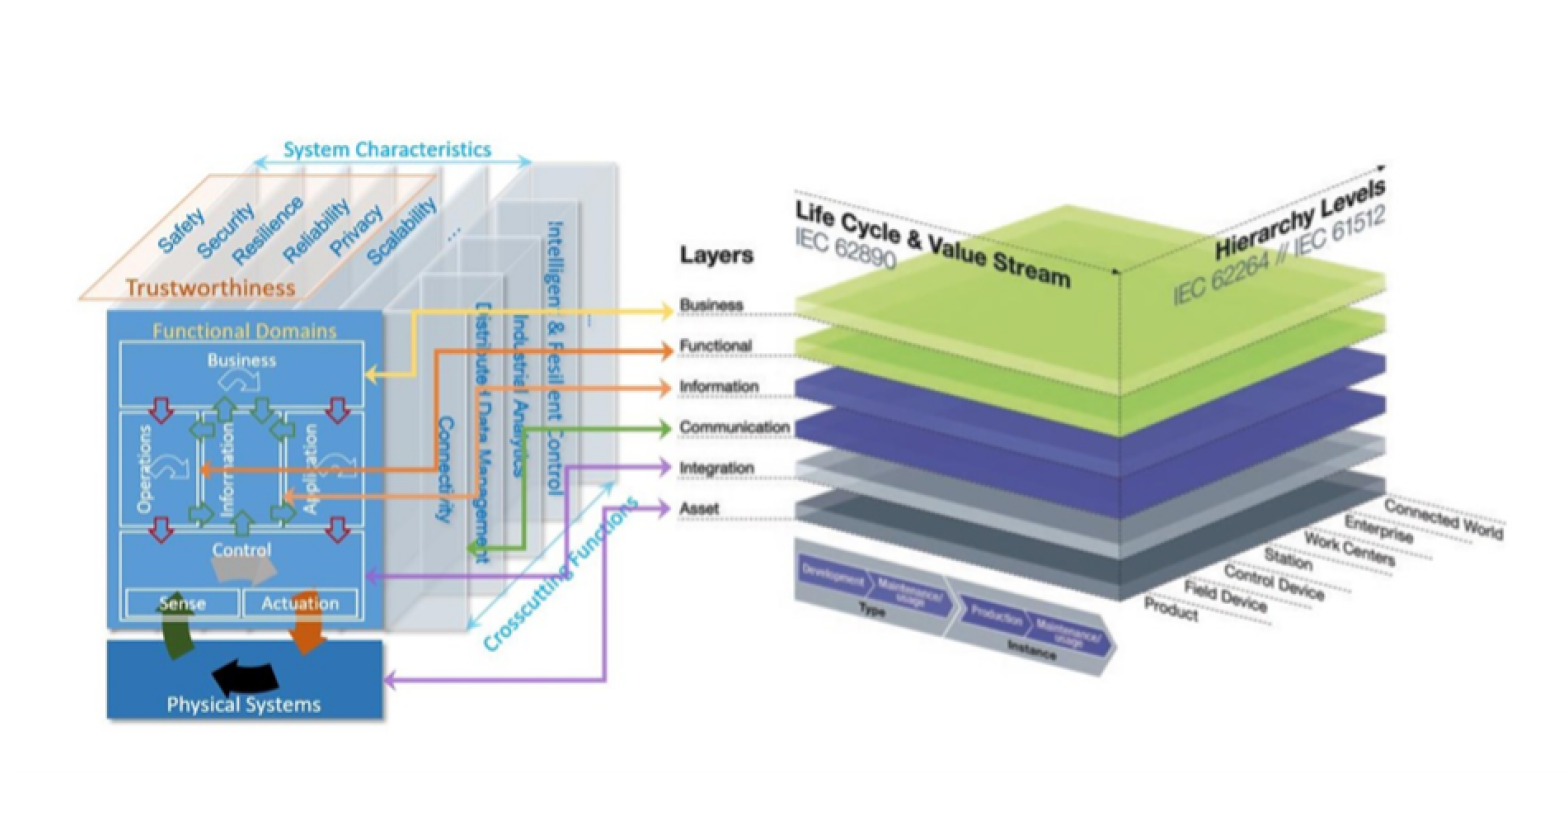
\includegraphics[width=0.7\linewidth]{Images/RAMI_IIRA.png}
		\caption{Mapping Functionalities in RAMI 4.0 and IIRA}
		\label{RAMI_IIRA}
	\end{center}
\end{figure}
  
These alignments ensure that SimplyTag analytics not only address Orgadata’s specific needs but also conform to global benchmarks, making them scalable and applicable across various industrial and urban contexts.
  
   
  
   

 